\documentclass[tikz,border=2pt]{standalone}
\usepackage{tikz}
\usepackage[european]{circuitikz}
\usetikzlibrary{arrows.meta,positioning,calc}
../cictikz/src/cictikz/data/tex/cictikz_lib.tex
\begin{document}
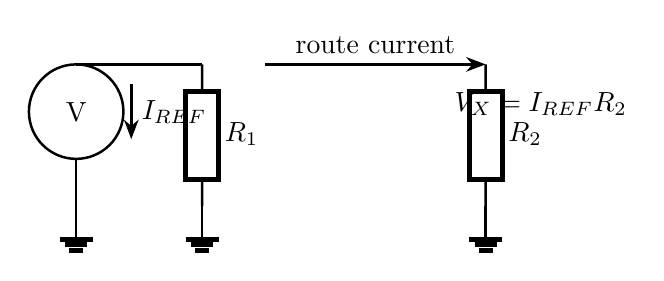
\begin{tikzpicture}[>=Stealth, line width=0.9pt]
  \draw (0,0) circle (0.6) node {V};
  \draw (0,-0.6) -- (0,-1.2) node[ground] {};
  \draw (0,0.6) -- (1.6,0.6);
  \draw (1.6,0.6) to[resistor,l=$R_1$] (1.6,-1.2) node[ground] {};
  \draw[->] (0.7,0.35) -- (0.7,-0.35) node[midway,right] {$I_{REF}$};

  \draw[->] (2.4,0.6) -- (5.2,0.6) node[midway,above] {route current};
  \draw (5.2,0.6) to[resistor,l=$R_2$] (5.2,-1.2) node[ground] {};
  \node at (5.9,0.1) {$V_X = I_{REF}R_2$};
\end{tikzpicture}
\end{document}
